\section{Parallelism in OpenMP}

The OpenMP standard is jointly defined by a group of major computer hardware
and software vendors\cite{Ope05}. This makes it a portable, scalable model that
gives shared-memory parallel programmers a simple and flexible interface for
developing parallel applications for platforms ranging from the desktop to the
supercomputer. The most powerful semantics in the standard is represented by a
\emph{parallel construct}. We will first look at mapping a parallel
construct onto a Cell processor.

%Memory model, and a parallel region

\subsection{A \texttt{parallel} region}

There are two types of processors in a Cell chip. The first type of processor
element, the PPE, is a 64-bit PowerPC Architecture core. It is fully compliant
with the 64-bit PowerPC Architecture and can run 32-bit and 64-bit operating
systems and applications. The second type of processor element, the SPE, is
optimized for running compute-intensive applications.  The SPEs are independent
processors, each running its own individual application program. Each SPE has
full access to coherent shared memory through DMA, including the memory-mapped
I/O space. The designation \emph{synergistic} for this processor was chosen
carefully because there is a mutual dependence between the PPE and the SPEs.
The SPEs depend on the PPE to run the operating system, and, in many cases, the
top-level control thread of an application. The PPE depends on the SPEs to
provide the bulk of the application performance. This dependency is reflected
in our OpenMP standard implementation: the sequential part of the program will
be executed by the PPU, and the parallel part, i.e., \texttt{parallel} regions,
of the program will be executed by the SPUs.  In this way, the user program can
take full advantage of the variety of PPU system libraries, while the SPEs will
help when the program is within the computationally intensive part.

This implementation scheme brings some challenges to the compiler
system, including: compiling for both PPU and SPU, switching between 
PPU and SPU execution, separating PPU libraries from SPU ones, and more.
We will cover some of these topics in this paper.

From a memory system point of view, the OpenMP standard specifies a
relaxed-consistency, shared-memory model. This model allows each thread to have
its own temporary view of memory. A value written to a variable, or a value
read from a variable, can remain in the thread's temporary view until it is
forced to share memory by an OpenMP flush operation. This memory model can be
efficiently implemented on the Cell memory structure, even though each SPE has
just 256K of directly accessible local memory for code, data, stack and heap.
In order to handle such limited memory, we only allocate private variables
accessed in SPE code in the SPE local store. Shared variables reside in system
memory, and SPE code can access them through DMA operations using either a DMA
buffer mechanism or software cache.

We set up the outermost parallel region by specifying the starting thread and
slave threads on the PPU and the SPUs separately. Nested parallel regions will
be executed on SPUs only. We still honor OpenMP data scoping clauses, using the
encountering threads to execute the nested parallel region sequentially.

%We only support one level of parallelism in the OpenMP standard.

\subsection{The \texttt{if} clause}

The \texttt{if} clause on a \texttt{parallel} region is useful when 
it is not known at compile time that
the computation part in a \texttt{parallel} region is
intense enough to outweigh the overhead of communication involved. For example,
the following code will be parallel executed on SPUs only when we have a large
enough loop bound.

{\small
\begin{verbatim}
   #pragama omp parallel for if (n>LIMIT)
   for (int i=0; i<n; i++) {
     compute(i); 
   }
\end{verbatim}
}

This could be rewritten as, (although it is equivalent in OpenMP 2.5, it may
not be true considering nested parallel regions in OpenMP 3.0)

{\small
\begin{verbatim}
   if (n>LIMIT) {
     #pragama omp parallel for 
     for (int i=0; i<n; i++) {
       compute(i); 
     }
   } else {
     compute(i); 
   }
\end{verbatim}
}

to avoid overhead for starting up
a parallel region. The function \texttt{compute} may be executed on
either the PPU or multiple SPUs. In such a case, the compiler have to
\emph{clone} the procedure for two different ISAs. We need to redraw
the Figure \ref{fig:runtime} as Figure \ref{fig:clone}.

\begin{figure}[!h]
  \begin{center}
    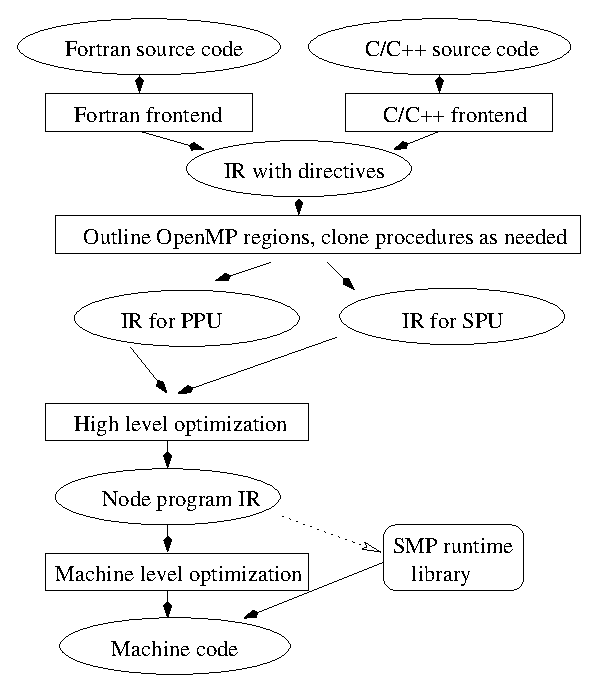
\includegraphics[angle=0, width=0.65\textwidth]{clone.eps}
    \caption{\footnotesize Clone for two ISAs}
    \label{fig:clone}
  \end{center}
\end{figure}

After we outline the parallel sections into procedures for an OpenMP region,
call graph analysis is needed within the compiler to trace which functions can
be reached from PPU and/or SPU. We then need to \emph{clone}, make two versions
of, the routine if a procedure will be reached by both PPU and SPU sides. The
SPU code is generated with the SPU linker, as a single SPU program executable.
The PPU code is also generated with the SPU program \emph{embedded} and linked
into the final PPU executable.

\subsection{The \texttt{num\_threads} clause}

According to the OpenMP standard, the thread which first encounter a parallel
construct becomes the master thread of a new team, with the thread number as
zero for the duration of the \texttt{parallel} region. Initially we did put the
PPU part of the parallel region. Experiments later on have shown some drawbacks
with this approach.

\begin{itemize}

\item The difference in computation power between a PPU and an SPU makes
  the PPU thread less useful in a workshare of the \texttt{parallel}
  region. We can not see any benchmarks benefit from assigning partial
  work to a PPU thread. The PPU thread may actually slow down the application,
  with load balancing playing a role.

\item In order to solve the above problem, we have to apply special
  loop schedules to disable the PPU inside an OpenMP workshare. This
  conflicts with the basic idea in an OpenMP environment, i.e., the
  threads in a parallel region, including both the master and the slave
  threads, are as equal as possible.

\item Even when we don't have any workshare in a parallel region, the PPU
  participation means that the computation in the parallel region will
  be carried out by both PPU and SPU, and may have different
  floating point results. SPU single precision arithmetic is not
  fully IEEE-794 compliant.

\item If the PPU participates in a parallel region, it will force the compiler
  to clone all the procedures can be reached by a parallel region,
  even without an \texttt{if} clause. This will extend the compilation
  time and may cause certain optimizations, such as pointer analysis, to
  give up due to an artificially enlarged problem size.

\item This will also prevent a user from providing his/her own
  computation kernel in an SPU only format. If parallel regions are SPU
  only, an advanced user can compile a procedure with a
  software-cache-aware SPU compiler and link it into the OpenMP
  compiler generated code, as long as this procedure can only be reached from a
  parallel region (without an \texttt{if} clause).

\end{itemize}

We decided to have the PPU thread start a \texttt{parallel} region, then
suspend execution and resume after the \texttt{parallel} region. Inside the
\texttt{parallel} region, the \texttt{num\_threads} clause or OpenMP
internal control variables will be used to determine how many SPU threads will
participate, and one of them will be picked as the master thread. This is more
in keeping with the upcoming OpenMP 3.0 \cite{Ope08} task view, where the code
outside and inside a parallel region are considered as different tasks.

We also set up a upper limit for the number of SPU threads can be used, it will
be the maximum number of SPUs available on the system. The concept is the same
as the \texttt{OMP\_THREAD\_LIMIT} environment variable in OpenMP 3.0.


